\outlineSubframe{Formale Eigenschaften}

\begin{frame}{Eigenschaften von Algorithmen}{Grundlegendes}
    \begin{itemize}[<+->]
        \item \textbf{Finitheit} - Ein Algorithmus lässt sich in endlch vielen Schritten eindeutig beschreiben
        \item \textbf{Ausführbarkeit} - Jeder Einzelschritt muss tatsächlich ausführbar sein
        \item \textbf{Platzkomplexität} - Ein Algorithmus benötigt zu jedem Zeitpunkt nur endlich viel Speicherplatz
        \item \textbf{Terminierung} - Der Algorithmus benötigt eine endliche Anzahl von Schritten zur Ausführung
        \item \textbf{Determiniertheit} - Der Algorithmus muss bei gleichen Rahmenbedingungen das gleiche Ergebnis liefern
        \item \textbf{Determinismus} - Der nächste Schritt des Algorithmus ist zu jedem Zeitpunkt genau definiert
    \end{itemize}
\end{frame}

\begin{frame}{Effizienz von Algorithmen}{}
    \begin{itemize}
        \item Ergibt sich indirekt aus den Grundlegenden Eigenschaften
        \item Effizienz lässt sich über verschiedene Größen beschreiben:
        \begin{itemize}
            \item Speicherverbrauch
            \item Zeitverbrauch
        \end{itemize}
        \item Die sind jedoch oft Implementierungs- und Rechnerabhägig
        \item Deshalb wird mit formalisierten Modellen gearbeitet
        \item ...Mehr dazu im Kapitel "`Analyse"'
    \end{itemize}
    
    Vgl. \cite{ottmann2017}, S. 2f
\end{frame}

\outlineSubframe{Darstellungsformen}

\begin{frame}[fragile]{Ein kleines Beispiel}{Warum wir das überhaupt brauchen (Algorithmus siehe \cite{wiki:qrsqrt})}
\lstset{style=cpp}
\begin{onlyenv}<1|handout:0>
\begin{lstlisting}
float Q_rsqrt( float number ){
  long i;
  float x2, y;
  const float threehalfs = 1.5F;

  x2 = number * 0.5F;
  y  = number;
  i  = * ( long * ) &y;                       
  i  = 0x5f3759df - ( i >> 1 );                
  y  = * ( float * ) &i;
  y  = y * ( threehalfs - ( x2 * y * y ) );   
//y  = y * ( threehalfs - ( x2 * y * y ) );   
  return y;
}
\end{lstlisting}
\end{onlyenv}
\begin{onlyenv}<2>
\begin{lstlisting}
float Q_rsqrt( float number ) {
  long i;
  float x2, y;
  const float threehalfs = 1.5F;

  x2 = number * 0.5F;
  y  = number;
  i  = * (long*) &y;   // evil floating point bit level hacking
  i  = 0x5f3759df - ( i >> 1 );   // what the fuck?
  y  = *(float*) &i;
  y  = y*(threehalfs-(x2*y*y));   // 1st iteration
//y  = y*(threehalfs-(x2*y*y));   // 2nd iteration, this can be removed
  return y;
}
\end{lstlisting}
\end{onlyenv}
\end{frame}

\begin{frame}{Warum wir das brauchen}
    \begin{itemize}[<+->]
        \item Source Code ist nicht immer verständlich
        \begin{itemize}
            \item Selbst mit Kommentaren...
        \end{itemize}
        \item Benötigt spezielles Wissen über die Sprache
        \item Nutzt ggf. Besonderheiten der Sprache aus
        \item Nutzt teilweise Workarounds (zum Beispiel aus Effizienzgründen)
    \end{itemize}
\end{frame}

\begin{frame}{Möglichkeiten der Darstellung}{}
    \begin{itemize}[<+->]
        \item Zur Definition von Algorithmen gibt es verschiedenste Möglichkeiten
        \item Mit ganz eigenen Vor- und Nachteilen
        \item Wir betrachten im Rahmen der Vorlesung:
        \begin{itemize}
            \item Prosatext
            \item Pseudocode
            \item Struktogramme
            \item Programmablaufplan (PAP)
        \end{itemize}
    \end{itemize}
\end{frame}

\begin{frame}{Was beschreiben wir?}{Unser Referenzalgorithmus}
    \begin{itemize}
        \item Um die verschiedenen Elemente zu vergleichen, wollen wir mit allen den folgenden Algorithmus beschreiben:
    \end{itemize}
    \pause
    \begin{alertblock}{Referenz}
        Für eine Zahl $n$ (Wobei gilt: $n \in \mathbb{N} $), soll die Summe aller geraden Zahlen von $0$ bis $n$ berechnet werden.
    \end{alertblock}
\end{frame}

\begin{frame}{Darstellung als Prosatext}{Der simple Weg}
    \begin{itemize}
        \item Simpelste Herangehensweise
        \item Man beschreibt in eigenen Worten, wie man vorgehen würde um die gegebene Problemstellung zu lösen
        \item \textbf{Achtung:} Unterscheiden zwischen Problemstellung und Lösungsbeschreibung!
        \item Auch in Prosaform sollten die Einzelschritte eindeutig beschrieben sein
        \item Nicht standardisiert $\rightarrow$ Beschreibung von Algorithmen inkonsistent
    \end{itemize}
\end{frame}

\begin{frame}{Prosabeschreibung}{An einem simplen Beispiel}
    \begin{alertblock}{Gebe alle Zahlen bis n aus}
    \visible<2->{Lese die Zahl \texttt{n} ein.}
    
    \visible<3->{Anschließend setze die Zählvariable \texttt{i} \texttt{0}.}
    
    \visible<4->{Gebe \texttt{i} aus.} \visible<5->{Erhöhe anschließend \texttt{i} um \texttt{1}.} \visible<6->{Wiederhole die letzten zwei Schritte bis \texttt{i} größer ist als \texttt{n}.}
    
    \visible<7->{Fertig.}
    \end{alertblock}
\end{frame}

\begin{frame}{Prosabeschreibung}{Für unseren Algorithmus}
    \begin{alertblock}{Addiere alle geraden Zahlen}
    \visible<2->{Lese die Zahl \texttt{n} ein.}
    
    \visible<3->{Anschließend setze die Zählvariable \texttt{i} sowie die Ergebnisvariable \texttt{res} auf \texttt{0}.}
    
    \visible<4->{Wenn \texttt{i} gerade ist, addiere \texttt{i} auf die Ergebnisvariable.} \visible<5->{Erhöhe anschließend \texttt{i} um \texttt{1}.} \visible<6->{Wiederhole die letzten zwei Schritte bis \texttt{i} größer ist als \texttt{n}.}
    
    \visible<7->{Gebe \texttt{res} aus}
    \end{alertblock}
\end{frame}

\begin{frame}{Darstellung als Pseudocode}{Der Zwischenweg}
    \begin{itemize}
        \item Mischung aus Prosa und tatsächlichem Code
        \item Orientiert sich an den in Programmiersprachen vorhandenen Strukturen (If-then-else, Schleifen...)
        \item Nutzt dabei aber leicht verständliche und programmiersprachenunabhängige Begriffe
        \item Wie Code in der Regel zeilenweise auf atomare Operationen beschränkt
        \item Keine formale Standardisierung, dadurch auch hier Inkonsistenzen möglich $\rightarrow$ Aber weniger als bei Prosabeschreibung
    \end{itemize}
\end{frame}

\begin{frame}[fragile]{Pseudocode}{An einem simplen Beispiel.}
\lstset{style=pseudo}
\begin{lstlisting}
LESE n
FUER i=0 BIS n
    WENN istPrim(i) DANN
        GEBE i AUS
    ENDE WENN
ENDE FUER
\end{lstlisting}
\end{frame}

\begin{frame}[fragile]{Pseudocode}{Für unser Pseudoproblem}
\lstset{style=pseudo}
\begin{onlyenv}
\begin{lstlisting}
LESE n
SETZE res=0
FUER i=0 BIS n
    WENN istGerade(i) DANN
        res+=i
    ENDE WENN
ENDE FUER
GEBE res AUS
\end{lstlisting}
\end{onlyenv}
\end{frame}

\begin{frame}{Struktogramme}{Der erste Standard}
    \begin{itemize}
        \item Entwickelt durch \textit{Nassi Shneidermann}
        \item Grafische Darstellung von Algorithmen
        \item Standardisiert nach \textbf{DIN 66261}
        \item Zerlegt den Algorithmus in elementare Grundstrukturen
        \item Die über die definierten Blöcke dargestellt werden
        \item Werden (lückenlos) von oben nach unten aneinander gereiht
    \end{itemize}
\end{frame}

\begin{frame}{Elemente von Struktogrammen}{Anweisung}
\begin{itemize}
    \item <+->Einzelne Anweisung:
\end{itemize}
\begin{onlyenv}<+->
\begin{centernss}
    \begin{struktogramm}(70,10)
        \assign{Einzelne Anweisung}
    \end{struktogramm}
\end{centernss}
\end{onlyenv}

\begin{itemize}
    \item <+-> Mehrere aufeinanderfolgende Anweisungen:
\end{itemize}
\begin{onlyenv}<+->
\begin{centernss}
    \begin{struktogramm}(70,30)
        \assign{Anweisung 1}
        \assign{Anweisung 2}
        \assign{Anweisung 3}
    \end{struktogramm}
\end{centernss}
\end{onlyenv}
\end{frame}

\begin{frame}{Elemente von Struktogrammen}{Verzweigungen}
\begin{itemize}
    \item <+->Einfache Verzweigung(if-then-else):
\end{itemize}
\begin{onlyenv}<+->
\begin{centernss}
\begin{struktogramm}(70,15)
        \ifthenelse[10]{3}{3}
            {x größer 5?}{True}{False}
            \assign[5]{Anweisung}
        \change
            \assign[5]{Else Anweisung}
        \ifend
    \end{struktogramm}
\end{centernss}
\end{onlyenv}
\begin{itemize}
    \item <+-> Mehrfache Verzweigung(switch-case):
\end{itemize}
\begin{onlyenv}<+->
\begin{centernss}
    \begin{struktogramm}(70,15)
        \case[10]{5}{3}{Wert von x?}{1}
            \assign{A}
        \switch{7}
            \assign{B}
        \switch{Default}
            \assign{C}
        \caseend
    \end{struktogramm}
\end{centernss}
\end{onlyenv}
\end{frame}

\begin{frame}{Elemente von Struktogrammen}{Zählschleifen}
\begin{itemize}
    \item <+->Einfache Zählschleifen(for-loop):
\end{itemize}
\begin{onlyenv}<+->
\begin{centernss}
\begin{struktogramm}(70,20)
    \while{von 0 bis 10, Schrittweite 2}
        \assign{Anweisungen}
    \whileend
\end{struktogramm}
\end{centernss}
\end{onlyenv}
\end{frame}

\begin{frame}{Elemente von Struktogrammen}{Schleifen}
\begin{itemize}
    \item <+->Kopfgeprüfte Schleifen(while):
\end{itemize}
\begin{onlyenv}<+->
\begin{centernss}
\begin{struktogramm}(70,20)
    \while{x>5}
        \assign{Anweisungen}
    \whileend
\end{struktogramm}
\end{centernss}
\end{onlyenv}

\begin{itemize}
    \item <+->Fußgeprüfte Schleifen(do-while):
\end{itemize}
\begin{onlyenv}<+->
\begin{centernss}
\begin{struktogramm}(70,20)
    \until{x>5}
        \assign{Anweisungen}
    \untilend
\end{struktogramm}
\end{centernss}
\end{onlyenv}
\end{frame}

\begin{frame}{Struktogram Beispiel}
\begin{centernss}
\begin{struktogramm}(100,75)
    \assign{Lese \( n \) ein}
    \assign{Setze \( res \) auf \( 0 \)}
    \until{n>0}
        \ifthenelse{3}{3}
            {\( i \) ist prim?}{Ja}{Nein}
            \assign{\( res+=i \)}
            \change
        \ifend
        \assign{Verringere \( n \) um \() 1 \) }
    \untilend
    \assign{Gebe \( res \) aus}
\end{struktogramm}
\end{centernss}
\end{frame}

\begin{frame}{Struktogram für unseren Algorithmus}
\begin{centernss}
\begin{onlyenv}
\begin{struktogramm}(100,75)
    \assign{Lese \( n \) ein}
    \assign{Setze \( res \) auf \( 0 \)}
    \while{von \( i=0 \) bis \( n \) }
        \ifthenelse{3}{3}
            {\( i \) ist gerade?}{Ja}{Nein}
            \assign{\( res+=i \)}
            \change
        \ifend
    \whileend
    \assign{Gebe \( res \) aus}
\end{struktogramm}
\end{onlyenv}
\end{centernss}
\end{frame}

\begin{frame}{Programmablaufplan}{Der zweite Standard}
    \begin{itemize}
        \item Bildet einen linearen Programmfluss aber
        \item Standardisiert nach \textbf{DIN 66001}
        \item Wie beim Struktogramm gibt es fest definierte Grundblöcke
        \item Diese werden hier jedoch über Pfeile verbunden
    \end{itemize}
\end{frame}

\begin{frame}{Elemente von Programmablaufplänen}{Start, Stop, Anweisungsblock, Ein- und Ausgaben}
\begin{figure}
    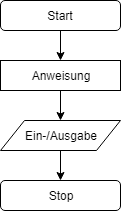
\includegraphics[height=5cm]{graph/pap_basics}
\end{figure}
\end{frame}

\begin{frame}{Elemente von Programmablaufplänen}{Verzweigungen}
\begin{figure}
    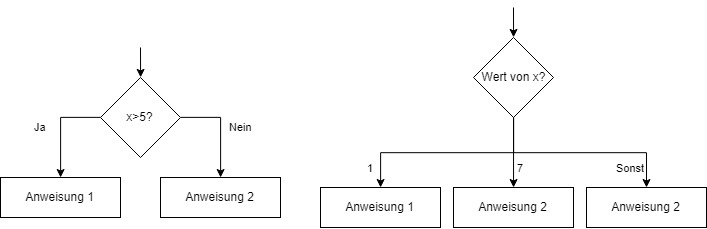
\includegraphics[width=0.9\textwidth]{graph/pap_decision}
\end{figure}
\end{frame}



\begin{frame}{Elemente von Programmablaufplänen}{Schleifen}
\begin{figure}
    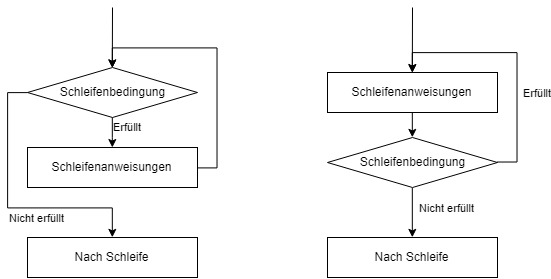
\includegraphics[height=5cm]{graph/pap_loops}
\end{figure}
\end{frame}

\begin{frame}{Elemente von Programmablaufplänen}{Zählschleifen}
\begin{figure}
    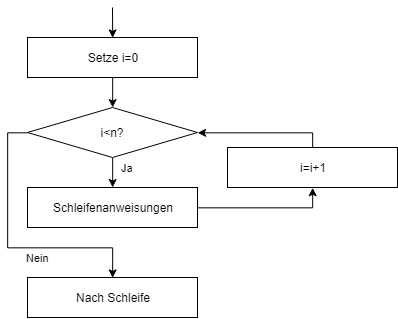
\includegraphics[height=5cm]{graph/pap_forloop}
\end{figure}
\end{frame}

\begin{frame}{Programmablaufplan}{...für unseren Algorithmus}
\begin{onlyenv}
\begin{figure}
    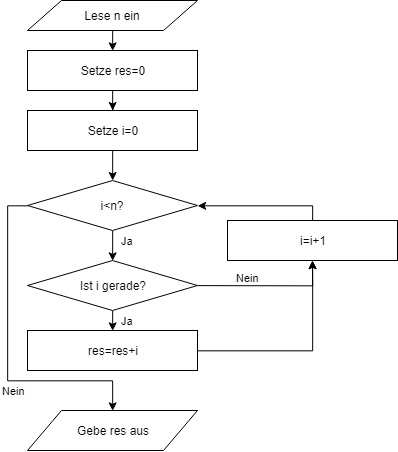
\includegraphics[height=5cm]{graph/pap_sumeven}
\end{figure}
\end{onlyenv}
\end{frame}

\begin{frame}{Zusammenfassung}
    \begin{itemize}[<+->]
        \item Keine der dargestellten Formen ist optimal
        \item Verwendung kommt auf Anforderungen und persönliche Vorlieben an
        \item Keine der hier vorgestellten Methoden zur Abbildung komplexerer objektorientierter Zusammenhänge möglich
        \item Weitere Darstellungsformen:
        \begin{itemize}
            \item Aktivitätsdiagramm
            \item Petrinetze
            \item Interaktionsdiagramme
        \end{itemize}
    \end{itemize}
\end{frame}